\documentclass[journal]{IEEEtran}
% ---------------------------------------------------------------------------
% Overleaf: set the compiler to pdfLaTeX (Menu -> Compiler). IEEEtran.cls and
% IEEEtran.bst are built into Overleaf; local copies are included in the zip.
% Every number in this draft comes from results/paper/paper_numbers.json and the
% gate files of the analysis pipeline. Items marked TODO need your input.
% ---------------------------------------------------------------------------
\usepackage{cite}
\usepackage{amsmath,amssymb}
\usepackage{graphicx}
\usepackage{booktabs}
\usepackage{multirow}
\usepackage{url}
\usepackage{xcolor}
\usepackage{tikz}
\usetikzlibrary{positioning,arrows.meta,fit}
\newcommand{\drand}{\Delta_{\mathrm{rand}}}
\newcommand{\dsig}{\Delta_{\mathrm{raw}}}
\newcommand{\ddemo}{\Delta_{\mathrm{demo}}}
\newcommand{\todo}[1]{\textcolor{red}{[TODO: #1]}}
\hyphenation{bio-metric bio-metrics electro-cardio-gram}

\begin{document}

\title{ECG Biometric Templates Leak Diagnoses: A Controlled Measurement Against Untrained, Signal, and Demographic Baselines}

\author{\todo{Author Name}, \todo{Co-author Name}, and \todo{Supervisor Name}%
\thanks{\todo{Affiliation, e.g., Department of \ldots, Indian Institute of Technology Roorkee, India. Corresponding author e-mail.}}%
\thanks{\todo{Funding statement, or remove.}}}

\markboth{\todo{Journal name}, Vol.~XX, No.~X, 2026}{\todo{Surname} \MakeLowercase{\textit{et al.}}: ECG Biometric Templates Leak Diagnoses}

\maketitle

\begin{abstract}
Electrocardiogram (ECG) biometrics store a compact template of a person's heartbeat to verify identity. Prior work has shown that identity-style training yields health-predictive ECG features, but it has not measured how much \emph{diagnostic} information a working biometric template exposes beyond what any network, the raw signal, or basic demographics already reveal. We train a CNN--Transformer identity encoder with ArcFace on lead~I of PTB-XL (1{,}689 training identities; equal error rate 0.059 on 422 unseen identities, versus 0.190 for a median-beat matcher), freeze it, and let an attacker predict diagnoses from templates of 3{,}372 patients the encoder never saw, in a lockbox test opened once under pre-registered rules. For conduction disturbance, the template exceeds five untrained copies of the same network by $\drand=+0.028$ AUROC (95\% CI 0.020--0.038; $p\le0.001$ against every copy), exceeds the raw median beat by $+0.044$, and adds $+0.130$ beyond age and sex. All four diagnostic superclasses leak after false-discovery-rate correction. Leakage rises as the biometric improves (Spearman $\rho=-0.75$ between identity error and leakage across checkpoints, $p=0.007$), persists across training seeds, a second lead, three attacker families and a Siamese biometric, and transfers to 1{,}055 patients of the Brazilian CODE-15\% cohort without retraining ($\drand=+0.021$, 95\% CI 0.007--0.038). ECG biometric templates should therefore be treated as health data.
\end{abstract}

\begin{IEEEkeywords}
Electrocardiogram, biometrics, privacy, information leakage, template protection, representation learning, PTB-XL.
\end{IEEEkeywords}

\section{Introduction}
\IEEEPARstart{T}{he} electrocardiogram (ECG) is a promising biometric: it is hard to spoof, always present, and recordable from a single lead by wearables and smartwatches~\cite{odinaka2012ecg}. Like a fingerprint system, an ECG biometric stores a \emph{template}, a fixed-length vector computed from the signal, and compares new recordings against it. Unlike a password hash, a template must preserve whatever makes one heart different from another. Some of those differences are caused by disease.

This raises a privacy question that the literature has approached only from the side. Representation-learning studies have shown that training ECG encoders to tell patients apart produces features that transfer well to clinical prediction~\cite{diamant2022pclr,sangha2024bcl,thiebaud2026biomecg}. Security studies have shown that hand-crafted ECG authentication features can expose health attributes~\cite{noh2022broken}, and that EEG biometric templates can leak medical information~\cite{holler2018eeg}. Neither line of work answers the question a data-protection officer would ask about a deployed system: \emph{if this biometric's stored templates are stolen, how much more diagnostic information does the thief obtain than they could already get without the biometric?}

Answering this requires three baselines. Untrained networks already produce features that predict diagnoses well, so an architecture-matched random baseline is needed~\cite{berger2026position}. The raw signal is the ceiling an attacker without the model could reach. Age and sex are freely available proxies of cardiovascular risk. We define leakage as the gain of the template over each baseline, measure it on patients the biometric never saw, and fix all analysis rules before the test set is opened.

Our contributions are:
\begin{enumerate}
\item A controlled leakage measure for biometric templates, $\drand$, $\dsig$ and $\ddemo$, evaluated on unseen patients with a sealed, pre-registered lockbox test (Section~\ref{sec:threat}).
\item Evidence that a working single-lead ECG biometric leaks all four PTB-XL diagnostic superclasses beyond an untrained copy of itself, with the largest leak for conduction disturbance (Section~\ref{sec:results}).
\item Evidence of a utility--leakage coupling: the better the biometric, the larger the leak.
\item Robustness across seeds, leads, attackers and biometric training objectives, and external transfer to a second population and recording system.
\item A repaired attribution-overlap test that, unlike our earlier heuristic, can fail, and here supports a shared signal basis for identity and diagnosis.
\end{enumerate}

\section{Related Work}
\subsection{ECG Biometrics}
ECG identification and verification have been studied for two decades, with comparative analyses of fiducial and non-fiducial features~\cite{odinaka2012ecg} and, more recently, deep encoders trained with metric-learning losses such as ArcFace~\cite{deng2019arcface} or Siamese contrastive objectives~\cite{hadsell2006dimensionality}. ElectroCardioGuard~\cite{sejak2023electrocardioguard} uses PTB-XL patient identity to detect misfiled records. These works optimise identification accuracy; they do not measure what else the templates reveal.

\subsection{Identity-Trained ECG Representations and Health}
Patient contrastive learning (PCLR)~\cite{diamant2022pclr} pre-trains ECG encoders by pulling together recordings of the same patient and shows strong downstream clinical performance. Biometric contrastive learning~\cite{sangha2024bcl} applies the same idea to ECG images. BiomECG~\cite{thiebaud2026biomecg} trains a Siamese biometric with cross-session evaluation and transfers frozen features to mortality, age and sex prediction, comparing against models trained from scratch. These studies establish that identity-style training yields health-relevant features, framed as a \emph{benefit}. None compares a working biometric against frozen untrained copies, the raw signal and demographics on unseen patients, nor frames the result as a privacy leak.

\subsection{Privacy Leakage from Biometric Templates}
H\"oller and Uhl~\cite{holler2018eeg} asked whether EEG biometric templates threaten user privacy. Noh \emph{et al.}~\cite{noh2022broken} analysed health-attribute leakage from ECG authentication features, and Kang \emph{et al.}~\cite{kang2023gan} proposed GAN-based hiding of patient information in an ECG authentication system. Our work differs in measuring leakage from a deep metric-learning template on unseen patients against architecture-, signal- and demographic-matched baselines, and in testing how leakage scales with biometric quality.

\subsection{Baselines for Representation Evaluation}
Berger \emph{et al.}~\cite{berger2026position} argue that ECG representation evaluations must include random-encoder baselines, because untrained networks already score highly. We adopt this as our primary comparator and make it architecture-matched and multi-seed.

\section{Threat Model and Leakage Measures}\label{sec:threat}
A service enrols users with an ECG biometric and stores their templates $t=f_\theta(x)$, where $f_\theta$ is the identity encoder and $x$ a lead-I recording. An attacker obtains the template database and, as is realistic, either the encoder or its templates for a small labelled auxiliary cohort (for example, from a public dataset). The attacker trains a classifier $g$ to predict a diagnosis $y$ from templates and applies it to the stolen ones. The attacker never sees the victims' raw signals.

Let $\mathrm{AUROC}(r)$ denote the test AUROC of the attacker using representation $r$. We define
\begin{align}
\drand &= \mathrm{AUROC}(f_\theta) - \frac{1}{K}\sum_{k=1}^{K}\mathrm{AUROC}(f_{\theta_k^0}),\label{eq:drand}\\
\dsig &= \mathrm{AUROC}(f_\theta) - \mathrm{AUROC}(\bar{b}),\\
\ddemo &= \mathrm{AUROC}(f_\theta \oplus d) - \mathrm{AUROC}(d),
\end{align}
where $f_{\theta_k^0}$ are $K=5$ untrained copies of the same architecture with independent random initialisations, $\bar b$ is the raw median heartbeat, $d$ is age and sex, and $\oplus$ is concatenation. $\drand$ is the primary measure: it isolates what identity \emph{training} adds. A leak counts only if its 95\% confidence interval excludes zero.

\section{Methods}\label{sec:methods}
\begin{figure*}[!t]
\centering
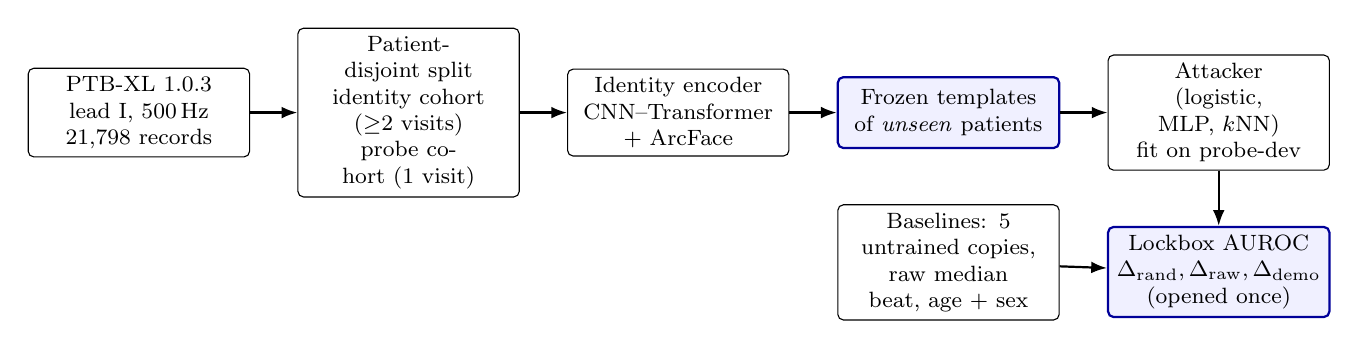
\begin{tikzpicture}[font=\footnotesize, node distance=4mm and 6mm,
  box/.style={draw, rounded corners=2pt, align=center, minimum height=9mm, inner sep=3pt, text width=26mm},
  key/.style={box, draw=blue!60!black, fill=blue!6, line width=0.8pt},
  arr/.style={-{Latex[length=2mm]}, thick}]
\node[box] (data) {PTB-XL 1.0.3\\lead I, 500\,Hz\\21{,}798 records};
\node[box, right=of data] (split) {Patient-disjoint split\\identity cohort ($\ge$2 visits)\\probe cohort (1 visit)};
\node[box, right=of split] (enc) {Identity encoder\\CNN--Transformer\\+ ArcFace};
\node[key, right=of enc] (tmpl) {Frozen templates\\of \emph{unseen} patients};
\node[box, right=of tmpl] (att) {Attacker\\(logistic, MLP, $k$NN)\\fit on probe-dev};
\node[box, below=7mm of tmpl] (base) {Baselines: 5 untrained copies,\\raw median beat, age + sex};
\node[key, below=7mm of att] (out) {Lockbox AUROC\\$\drand,\dsig,\ddemo$\\(opened once)};
\draw[arr] (data) -- (split); \draw[arr] (split) -- (enc); \draw[arr] (enc) -- (tmpl);
\draw[arr] (tmpl) -- (att); \draw[arr] (att) -- (out); \draw[arr] (base) -- (out);
\end{tikzpicture}
\caption{Study design. The identity encoder is trained only on patients with repeat visits; leakage is measured on single-visit patients it never saw, against three baselines. All rules were written to a dated file before the lockbox was opened.}
\label{fig:design}
\end{figure*}

\subsection{Data and Cohorts}
We use PTB-XL version 1.0.3~\cite{wagner2020ptbxl,goldberger2000physionet}: 21{,}799 10-s, 12-lead recordings from 18{,}869 patients. Every file was verified against PhysioNet's SHA-256 list (43{,}600/43{,}600 matched). Diagnostic SCP statements were mapped to five superclasses (NORM, MI, STTC, CD, HYP)~\cite{strodthoff2021deep}. We use lead~I, the lead available from wrist and smartwatch devices.

Signals were band-pass filtered (4th-order Butterworth, 0.5--40\,Hz, zero-phase) and $z$-scored per record. R-peaks were detected with NeuroKit2~\cite{makowski2021neurokit2}, and a median beat from $-250$ to $+400$\,ms around the R-peak (325 samples) was formed. One record failed quality control (implausible beat count), leaving 21{,}798.

Patients were split before any modelling (Table~\ref{tab:cohorts}). Patients with two or more recordings form the \emph{identity cohort}, divided 80/20 into identity-training and identity-evaluation identities. Single-recording patients form the \emph{probe cohort}, used only by the attacker: 70\% for attacker development (five patient-disjoint folds), stratified by label pattern, and 30\% as a \emph{lockbox} test. No patient appears in more than one split. Binary tasks compare each superclass against NORM-only records.

\begin{table}[!t]
\centering
\caption{Cohorts (PTB-XL 1.0.3, lead I, after quality control)}
\label{tab:cohorts}
\begin{tabular}{@{}lrrl@{}}
\toprule
Split & Records & Patients & Role \\
\midrule
Identity training & 4{,}047 & 1{,}689 & train biometric \\
Identity evaluation & 994 & 422 & unseen identities \\
Attacker development & 11{,}728 & 11{,}728 & fit attacker \\
Lockbox test & 5{,}029 & 5{,}029 & final test, once \\
\bottomrule
\end{tabular}\\[2pt]
\footnotesize Lockbox positives vs.\ NORM-only: CD 1{,}072/2{,}300; MI 1{,}124/2{,}300; STTC 1{,}102/2{,}300; HYP 583/2{,}300. \todo{Add age and sex per split from table1\_cohorts.csv (cell 6.2).}
\end{table}

\subsection{Identity Encoder}
The encoder maps a 2.5-s window (1{,}250 samples) to a 256-dimensional unit vector. Three convolutional blocks (kernel 7; 32, 64, 128 channels; batch normalisation, GELU, max-pooling) feed a two-layer Transformer encoder~\cite{vaswani2017attention} ($d=128$, four heads, learned positional embeddings), followed by mean pooling, a linear projection and $\ell_2$ normalisation. It is trained with ArcFace~\cite{deng2019arcface} ($s=30$, $m=0.5$) over identity-training patients using AdamW (learning rate $10^{-3}$, weight decay $10^{-4}$, cosine schedule with 5\% warm-up), batch size 128, random crops with $\pm10\%$ amplitude scaling and Gaussian noise, and mixed precision. Training stopped when identity-evaluation EER did not improve for 10 epochs. Diagnostic labels are never used. A record's template is the normalised mean of the embeddings of its four non-overlapping windows.

Verification is evaluated on identity-evaluation patients: each patient's earliest recording is enrolled and later recordings are verified against all enrolled patients. We report EER and rank-1 accuracy. A median-beat nearest-match matcher is the identity baseline. Before testing for leakage, we required the encoder's EER to be at most 0.8 times the baseline's.

\subsection{Attacker and Baselines}
The primary attacker standardises features and fits an $\ell_2$-regularised logistic regression, with the regularisation strength chosen from $\{10^{-3},\ldots,10^{2}\}$ by five-fold patient-disjoint cross-validation on attacker-development data. It is then refitted on all development data and applied once to the lockbox. The same attacker is applied to (i) the identity template, (ii) templates from each of five untrained copies (seeds 100--104, evaluation mode), (iii) the raw median beat reduced to 64 dimensions by PCA fitted on development data, (iv) age and sex, and (v) template plus age and sex. Secondary attackers are a one-hidden-layer MLP (256 units) and a distance-weighted $k$NN with $k$ chosen by cross-validation.

\subsection{Statistics}
Confidence intervals use 2{,}000 paired patient-bootstrap resamples of the lockbox, recomputing every AUROC on the same resample~\cite{efron1993bootstrap}. For the primary result, we additionally test the template against \emph{each} untrained copy with a paired permutation test (1{,}000 permutations, swapping the two models' rank-normalised scores within patients) and report the largest $p$. Secondary permutation tests compare against the rank-averaged ensemble of the five copies, which is a stronger and therefore conservative opponent. Across the four superclasses, $p$-values are corrected with the Benjamini--Hochberg procedure~\cite{benjamini1995controlling}.

\subsection{Pre-registration and Lockbox}
Before the main encoder was trained, the identity criterion, hypotheses, attacker and statistics settings were written to a dated plan file. The trained model's SHA-256 fingerprint was recorded before the lockbox was loaded, and the pipeline refuses to score the lockbox with any other model. The lockbox was scored once. Robustness analyses were specified in a second dated plan before they ran.

\subsection{Secondary Analyses}
\emph{Utility--leakage coupling (H3).} We retrained the encoder along the same 19-epoch trajectory, saved 11 snapshots, and measured identity EER and $\drand$ (cross-validated on development data, leaving the lockbox untouched) at each.

\emph{Persistence (H5).} In the identity cohort, persistence is the fraction of visits with a superclass whose next visit retains it. We relate it to each superclass's $\drand$.

\emph{Siamese biometric.} To test whether leakage depends on the training objective, we trained the same architecture with a contrastive pair loss~\cite{hadsell2006dimensionality}, analogous to the Siamese design of BiomECG~\cite{thiebaud2026biomecg}.

\emph{Attribution overlap (H4).} We trained a supervised CD diagnosis model and a copy on shuffled labels, and computed integrated gradients~\cite{sundararajan2017axiomatic} for 300 lockbox windows. For the identity model, the explained output is the similarity of a window to the record's own template. Overlap is the per-record Spearman correlation of absolute attributions over time, using raw values without min--max rescaling. It must exceed two nulls: identity vs.\ shuffled-label diagnosis, and untrained identity vs.\ diagnosis. The second null removes overlap that arises only because every model attends to the QRS complex.

\subsection{Robustness and External Validation}
We retrained the encoder with seeds 1 and 2, and repeated the full pipeline on lead~II, reusing lead-I R-peak positions. For external validation we used the first part of CODE-15\%~\cite{ribeiro2021code15,ribeiro2020automatic}, a Brazilian cohort recorded at 400\,Hz. We kept 10-s exams (7{,}699 of 20{,}001), used lead DI resampled to 500\,Hz with identical preprocessing, and defined a CD-equivalent label as right or left bundle branch block or first-degree AV block, against normal ECGs with none of the six annotated abnormalities. Using one exam per patient, we split 70/30 into attacker development (2{,}461 patients) and test (1{,}055 patients: 117 CD-equivalent, 938 normal). The PTB-XL encoder was applied frozen, without retraining.

\section{Results}\label{sec:results}
\subsection{The Biometric Works}
Table~\ref{tab:identity} summarises verification on identities never seen in training. The ArcFace encoder reached an EER of 0.059 (rank-1 0.633) against 0.190 (rank-1 0.432) for the median-beat matcher, passing the pre-registered criterion. Training took 19 epochs of about 4\,s each on an NVIDIA T4, with the best epoch at 9. The encoder transferred to CODE-15\% repeat patients without retraining (EER 0.156 vs.\ 0.204).

\begin{table}[!t]
\centering
\caption{Identity verification on unseen identities (lower EER is better)}
\label{tab:identity}
\begin{tabular}{@{}llcc@{}}
\toprule
Model & Data & EER & Rank-1 \\
\midrule
Median-beat matcher & PTB-XL lead I & 0.190 & 0.432 \\
ArcFace, seed 0 (primary) & PTB-XL lead I & \textbf{0.059} & \textbf{0.633} \\
ArcFace, seed 1 & PTB-XL lead I & 0.054 & -- \\
ArcFace, seed 2 & PTB-XL lead I & 0.060 & -- \\
Siamese contrastive & PTB-XL lead I & 0.068 & 0.538 \\
Median-beat matcher & PTB-XL lead II & 0.159 & -- \\
ArcFace & PTB-XL lead II & 0.054 & -- \\
Median-beat matcher & CODE-15\% (181 pts) & 0.204 & -- \\
ArcFace seed 0, frozen & CODE-15\% (181 pts) & 0.156 & 0.620 \\
\bottomrule
\end{tabular}
\end{table}

\subsection{Primary Result: Conduction Disturbance}
On the lockbox (1{,}072 CD vs.\ 2{,}300 NORM), the attacker reached AUROC 0.867 from identity templates, against 0.835--0.845 (mean 0.840) from the five untrained copies, 0.823 from the raw median beat and 0.758 from age and sex. This gives $\drand=+0.028$ (95\% CI 0.020--0.038), $\dsig=+0.044$ (0.029--0.058) and $\ddemo=+0.130$ (0.113--0.146). The template beat \emph{each} untrained copy individually (gains $+0.021$ to $+0.032$, all $p\le0.001$; bootstrap two-sided $p=0.0005$). Hypotheses H1 and H2 were supported under the pre-registered rules.

\subsection{All Diagnostic Superclasses Leak}
Table~\ref{tab:leakage} and Fig.~\ref{fig:leakage} report all four tasks. $\drand$ excluded zero for every superclass and remained significant after correction (CD $+0.028$, MI $+0.017$, HYP $+0.016$, STTC $+0.013$; corrected $p$ 0.002--0.017). $\dsig$ excluded zero for CD, MI and HYP but not for STTC, where the raw median beat alone already reaches AUROC 0.932. ST/T changes are directly visible in the beat morphology, leaving little for the template to add.

\begin{table*}[!t]
\centering
\caption{Diagnostic leakage on the lockbox (attacker: logistic regression; 95\% bootstrap CI; $p$ for $\drand$ Benjamini--Hochberg corrected)}
\label{tab:leakage}
\footnotesize\setlength{\tabcolsep}{3.5pt}
\resizebox{\textwidth}{!}{%
\begin{tabular}{@{}lccccccccc@{}}
\toprule
& & \multicolumn{4}{c}{AUROC} & & & & \\
\cmidrule(lr){3-6}
Task & Pos./Neg. & Template & Untrained (mean) & Raw beat & Age+sex & $\drand$ [95\% CI] & $\dsig$ [95\% CI] & $\ddemo$ [95\% CI] & $p_{\mathrm{BH}}$ \\
\midrule
CD vs.\ NORM & 1072/2300 & 0.866 & 0.838 & 0.823 & 0.758 & $+0.028$ [0.020, 0.038] & $+0.044$ [0.029, 0.058] & $+0.130$ [0.113, 0.146] & 0.002 \\
MI vs.\ NORM & 1124/2300 & 0.880 & 0.863 & 0.858 & 0.782 & $+0.017$ [0.010, 0.024] & $+0.022$ [0.012, 0.033] & $+0.122$ [0.108, 0.137] & 0.015 \\
STTC vs.\ NORM & 1102/2300 & 0.935 & 0.922 & 0.932 & 0.745 & $+0.013$ [0.008, 0.017] & $+0.003$ [$-$0.003, 0.008] & $+0.190$ [0.174, 0.207] & 0.002 \\
HYP vs.\ NORM & 583/2300 & 0.917 & 0.900 & 0.897 & 0.751 & $+0.016$ [0.008, 0.026] & $+0.020$ [0.007, 0.033] & $+0.174$ [0.154, 0.195] & 0.017 \\
\bottomrule
\end{tabular}}
\end{table*}

\begin{figure*}[!t]
\centering
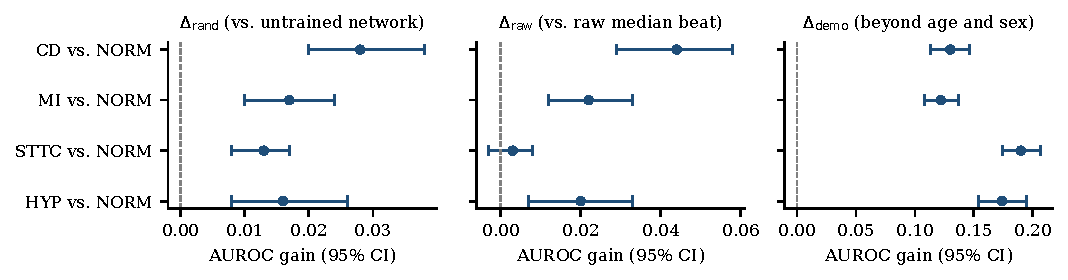
\includegraphics[width=\textwidth]{figures/fig_leakage.pdf}
\caption{Leakage for four diagnostic superclasses on the lockbox. Left: gain over five untrained copies of the encoder ($\drand$). Middle: gain over the raw median beat ($\dsig$). Right: gain of template plus demographics over demographics alone ($\ddemo$). Bars are 95\% patient-bootstrap CIs.}
\label{fig:leakage}
\end{figure*}

\subsection{A Better Biometric Leaks More}
Across 11 training snapshots, identity EER fell from 0.189 to 0.058--0.068 while $\drand$ (development data) rose from $+0.015$ to $+0.021$--$+0.025$ (Fig.~\ref{fig:coupling}a). The rank correlation between identity error and leakage was $\rho=-0.75$ ($p=0.007$), supporting H3. Even the first epoch leaked, which suggests that leakage appears as soon as the encoder starts separating individuals. Persistence and leakage were positively but not significantly related across the four superclasses ($\rho=+0.60$; Fig.~\ref{fig:coupling}b). With four points this is descriptive only (H5).

\begin{figure*}[!t]
\centering
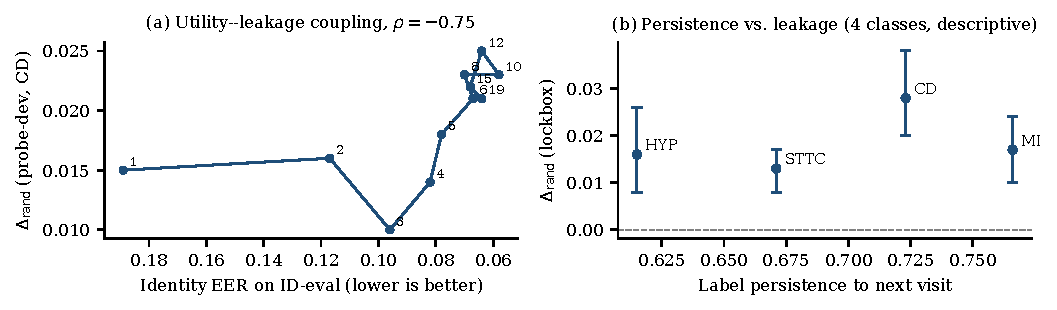
\includegraphics[width=\textwidth]{figures/fig_coupling.pdf}
\caption{(a) Identity error vs.\ CD leakage across 11 training snapshots (numbers are epochs); the $x$-axis is reversed so that better biometrics lie to the right. (b) Persistence of each superclass to the next visit vs.\ its lockbox $\drand$.}
\label{fig:coupling}
\end{figure*}

\subsection{Attackers, Biometric Objectives and Attributions}
A $k$NN attacker found a larger leak ($\drand=+0.046$, 95\% CI 0.034--0.058) and an MLP a smaller one ($+0.013$, 0.003--0.023; ensemble permutation $p=0.19$). The leak is present under every attacker, but its magnitude depends on the attacker; the linear estimate is neither the largest nor a strict lower bound. The Siamese contrastive biometric also leaked ($+0.017$, 0.010--0.025) at a similar identity quality (EER 0.068), so leakage is not specific to ArcFace.

Integrated-gradient attributions of the identity and diagnosis models overlapped more (mean per-record Spearman 0.579) than either null (0.501 for shuffled-label diagnosis; 0.509 for the untrained identity encoder). The excess was $+0.077$ (95\% CI 0.070--0.084) and $+0.070$ (0.065--0.074) respectively (Fig.~\ref{fig:attr}), supporting H4: identity and diagnosis rely on partly shared signal regions beyond the generic QRS emphasis.

\begin{figure}[!t]
\centering
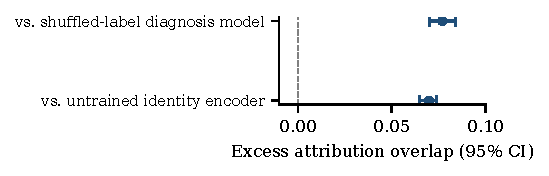
\includegraphics[width=\columnwidth]{figures/fig_attribution.pdf}
\caption{Excess attribution overlap between the identity encoder and a CD diagnosis model over two nulls (300 lockbox records; 95\% bootstrap CI).}
\label{fig:attr}
\end{figure}

\subsection{Robustness and External Validation}
The CD leak held in every robustness setting (Fig.~\ref{fig:robust}). Across three seeds, $\drand=+0.026\pm0.006$ (each CI excluding zero), $\dsig=+0.041\pm0.006$ and $\ddemo=+0.125\pm0.006$. On lead~II the leak was smaller but present ($\drand=+0.008$, 0.002--0.014; $\dsig=+0.034$; $\ddemo=+0.159$). On CODE-15\%, the frozen PTB-XL encoder leaked CD-equivalent disease beyond untrained copies ($\drand=+0.021$, 0.007--0.038) and beyond demographics ($\ddemo=+0.148$, 0.115--0.184). The gain over the raw beat was not significant there ($\dsig=+0.016$, $-0.013$--$0.047$).

\begin{figure}[!t]
\centering
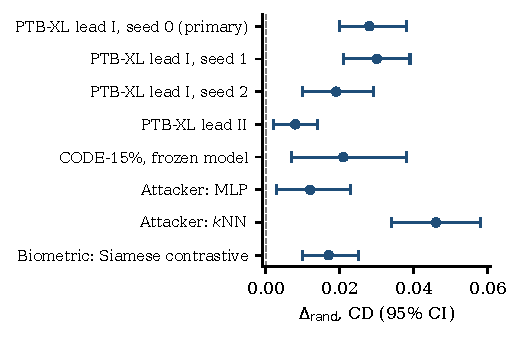
\includegraphics[width=\columnwidth]{figures/fig_robustness.pdf}
\caption{$\drand$ for CD (95\% CI) across training seeds, leads, attackers, biometric objective, and the external CODE-15\% cohort with the PTB-XL encoder frozen.}
\label{fig:robust}
\end{figure}

\section{Discussion}
\subsection{Templates Are Health Data}
A stolen ECG template gives an attacker diagnostic information they could not get from an untrained network, and for most diagnoses not even from the raw heartbeat. Because templates are designed to be stored and compared, often on servers or devices outside clinical control, they inherit a privacy risk usually associated with medical records. Where health data receives special protection, such as Article~9 of the EU General Data Protection Regulation~\cite{gdpr2016}, our findings argue that ECG templates should be assessed as potentially revealing health status. This is a technical observation, not a legal opinion.

\subsection{Why Templates Leak}
Two findings point to the mechanism. First, leakage grows with identity quality across training, so it is a by-product of learning what makes a heart individual rather than an accident of a particular checkpoint. Second, identity and diagnosis attributions overlap beyond both nulls. Conduction abnormalities alter QRS morphology in a way that is stable within a person, and such stable, person-specific features are exactly what a biometric is trained to keep. The weaker leak on lead~II, and the absence of a gain over the raw beat for STTC, are consistent with this view: when the raw morphology already exposes a diagnosis, the template adds little.

\subsection{Relation to Prior Work}
Our results agree with PCLR, biometric contrastive learning and BiomECG~\cite{diamant2022pclr,sangha2024bcl,thiebaud2026biomecg}, which report that identity-style training yields clinically useful features. We reframe that utility as a risk and measure it against frozen, architecture-matched untrained baselines~\cite{berger2026position} rather than models trained from scratch. Compared with analyses of hand-crafted ECG authentication features~\cite{noh2022broken}, we study learned metric-learning templates, unseen patients, and the dependence of leakage on biometric quality. Defences such as GAN-based information hiding~\cite{kang2023gan} are complementary, and our measures provide a way to evaluate them.

\subsection{Limitations}
The leaks are modest in absolute size ($+0.008$ to $+0.046$ AUROC). They are consistent and replicated, but they do not imply that templates alone allow reliable diagnosis. The external test is small (117 CD-equivalent test patients), and its gain over the raw beat is not significant. The H3 snapshots come from a single training trajectory and are not independent observations. H5 rests on four superclasses. Secondary permutation tests against the untrained ensemble are conservative and gave larger $p$-values than the bootstrap intervals (for example, MLP attacker, lead~II and CODE-15\%). We report both, and for the primary result we tested against every copy individually. Finally, we studied single-lead, 10-s resting ECGs; wearable recordings are noisier and may leak less or differently.

\subsection{Future Work}
Natural next steps are to quantify leakage at clinically meaningful operating points, test template-protection and information-hiding defences with the proposed measures, extend the external evaluation to more of CODE-15\%, and study wearable-grade signals.

\section{Conclusion}
A working ECG biometric template reveals diagnoses beyond what an untrained copy of the same network, the raw heartbeat or age and sex reveal. The leak covers all four PTB-XL diagnostic superclasses, grows as the biometric improves, and survives changes of seed, lead, attacker, training objective and population. ECG biometric systems should treat stored templates as sensitive health data and evaluate template protection against diagnostic, not only identity, attacks.

\section*{Data and Code Availability}
PTB-XL~\cite{wagner2020ptbxl} and CODE-15\%~\cite{ribeiro2021code15} are publicly available under CC BY 4.0. The analysis code, patient-level split identifiers, pre-registration files and gate records will be released at \todo{repository URL}.

\section*{Acknowledgment}
\todo{Acknowledge supervisor, institution, and compute (Google Colab).}

\bibliographystyle{IEEEtran}
\bibliography{references}

\end{document}
